\frame{
    \frametitle{Coupling Interpolation Through NNT Direct Combination}
    \begin{columns}
        \begin{column}{0.4\textwidth}
            \begin{center} 
            {\tiny NNT Basis Set}

            \resizebox{0.2\textheight}{!}{ \begin{tabular}{ |l|l|l| }
                \hline
                \textbf {$\kappa_{2V}$} & \textbf {$\kappa_\lambda$} & \textbf {$\kappa_V$} \\
                \hline
                    1.  &   1. & 1.  \\
                    2.  &   1. & 1.  \\
                    1.5 &   1. & 1.  \\
                    0.  &   1. & 0.5 \\
                    1.  &   0. & 1.  \\
                    1.  &  10. & 1.  \\
                \hline
            \end{tabular}}
            \end{center}

        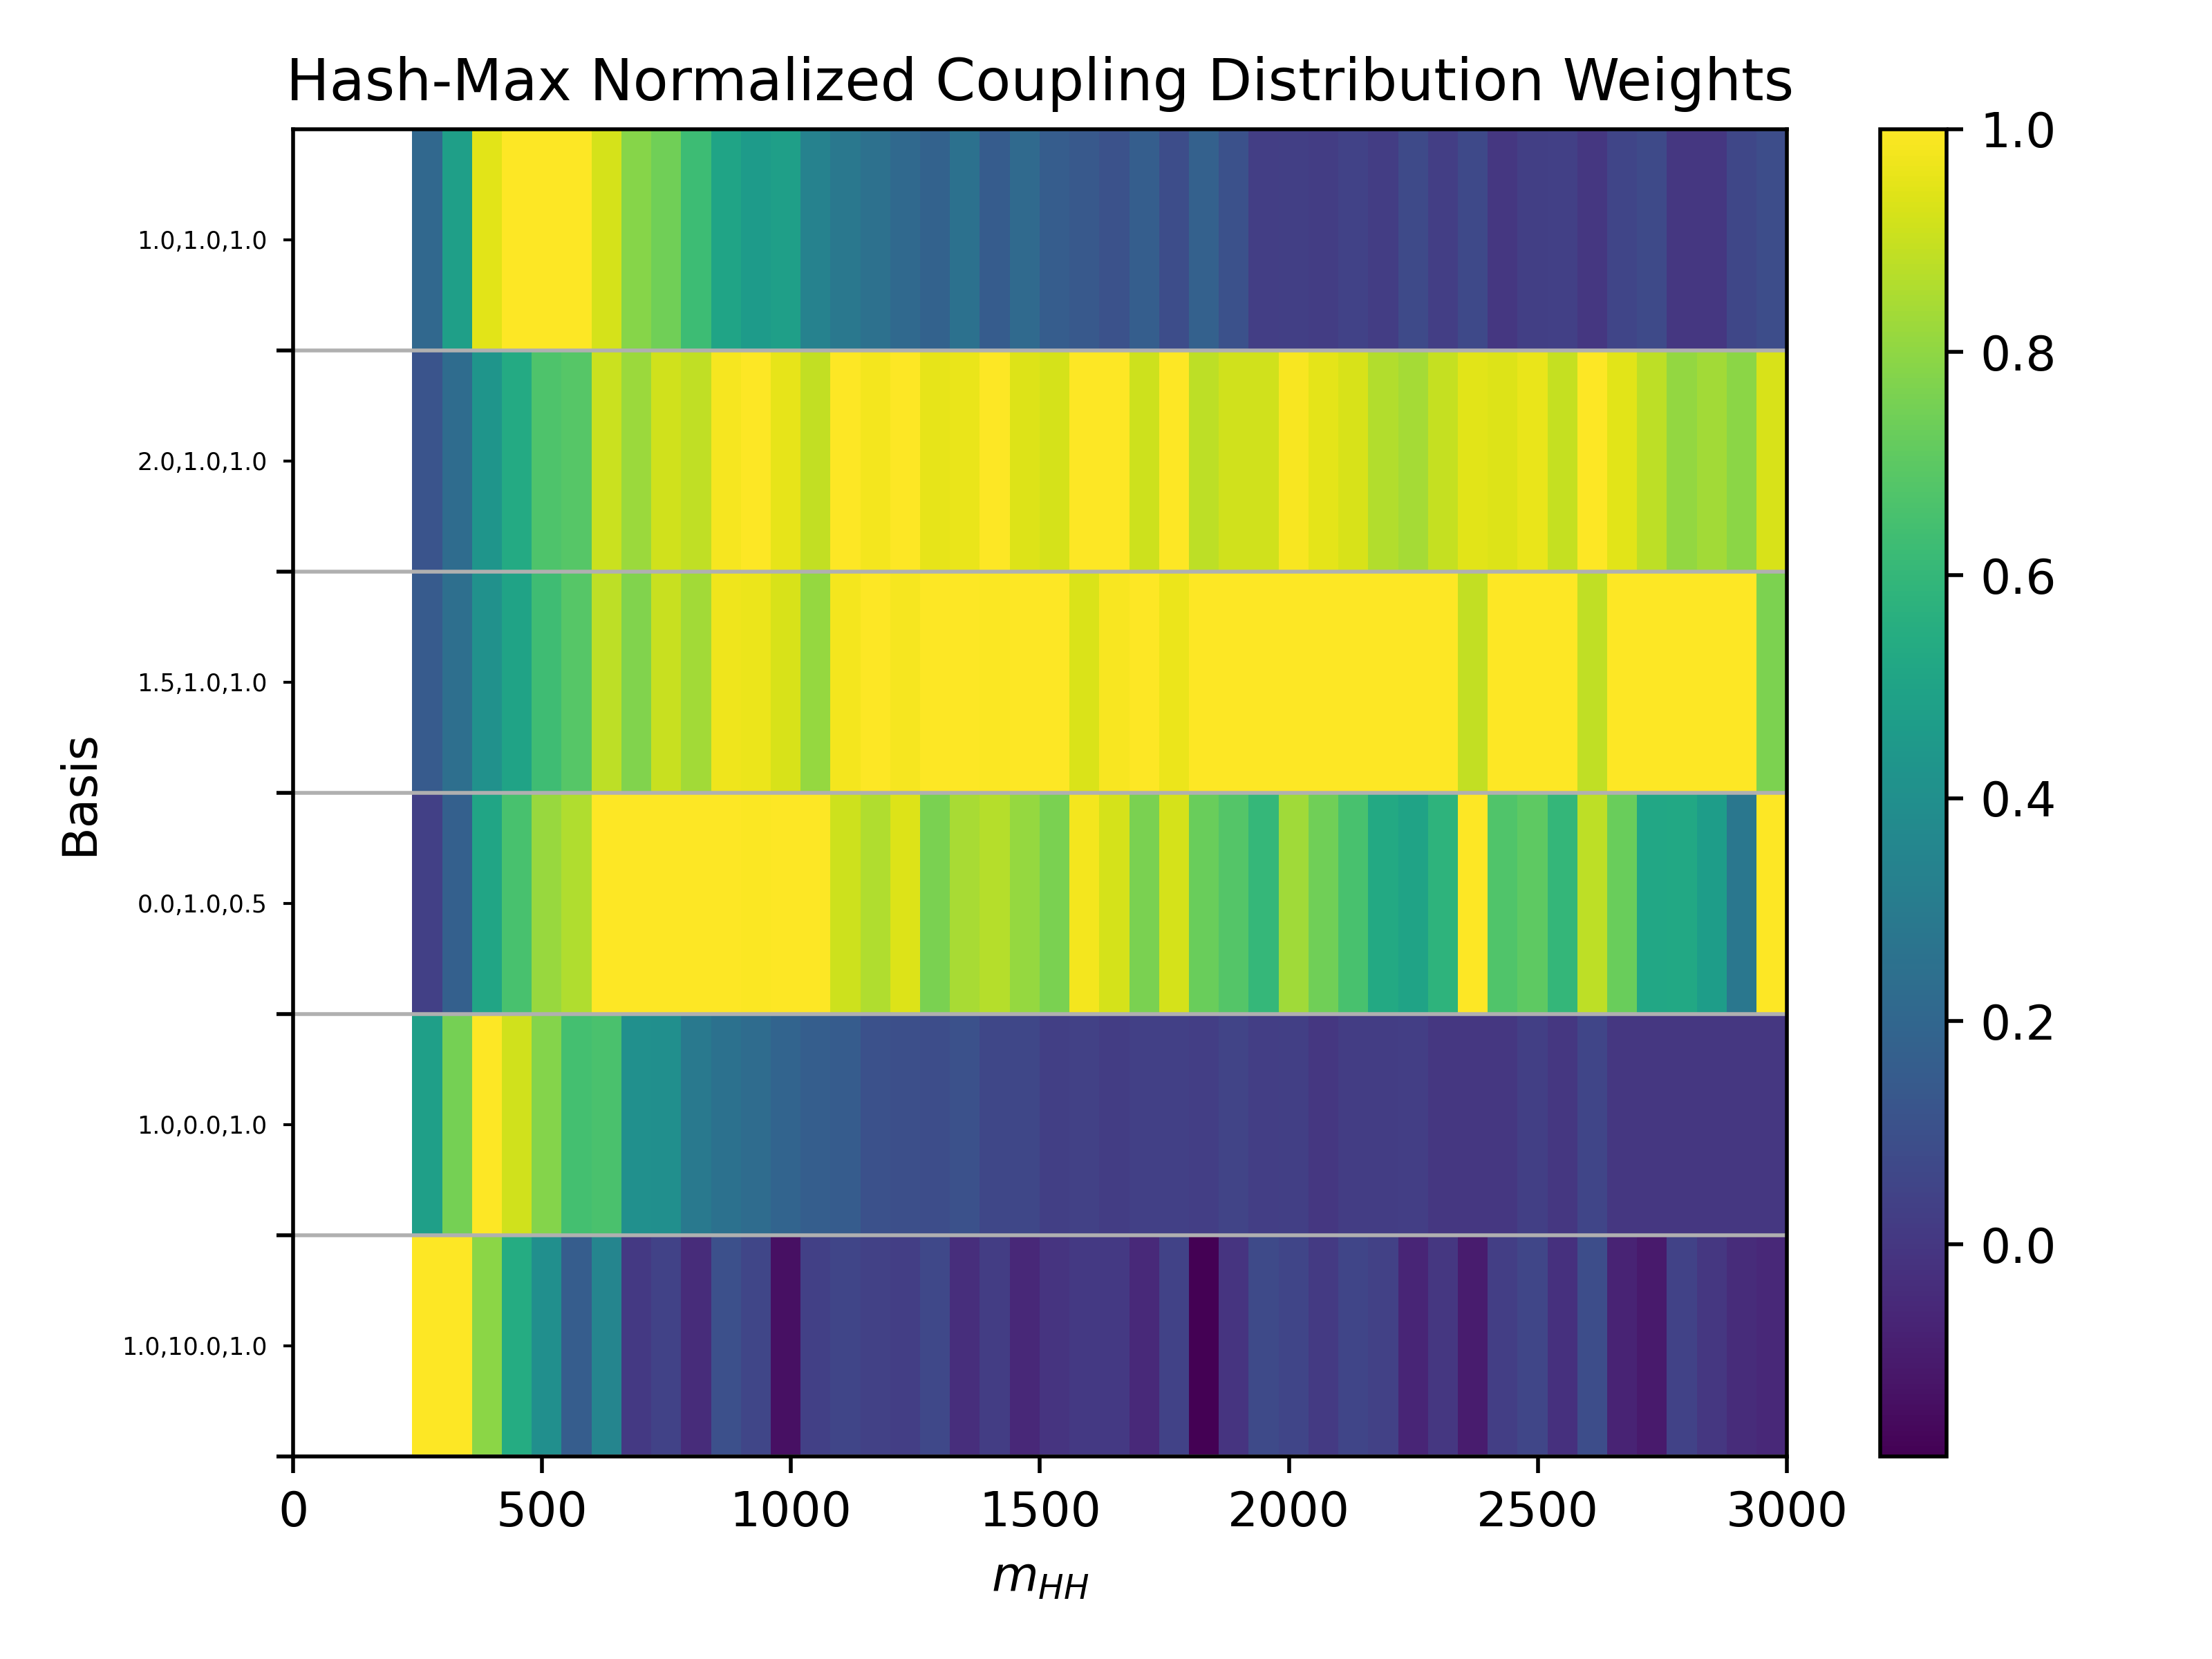
\includegraphics[width=\linewidth,height=\textheight,keepaspectratio]
            {coupling_scan_auto_chosen_reco_R0_hash_max}

        \end{column}
        \begin{column}{0.6\textwidth}
            \resizebox{0.8\textwidth}{!}{ \begin{minipage}{1.0\textwidth}
            Linear Combination Equation

            \vspace{10mm}

            {\tiny $
    \left(2 \kappa_{2V}^{2} - \frac{124 \kappa_{2V} \kappa_{V}^{2}}{9} + \frac{61 \kappa_{2V} \kappa_{V} \kappa_{\lambda}}{9} + \frac{106 \kappa_{V}^{4}}{9} - \frac{17 \kappa_{V}^{3} \kappa_{\lambda}}{3} - \frac{\kappa_{V}^{2} \kappa_{\lambda}^{2}}{9}\right) \left|{A{\left(1,1,1 \right)}}\right|^{2} +
$

$
    \left(2 \kappa_{2V}^{2} - 8 \kappa_{2V} \kappa_{V}^{2} + 3 \kappa_{2V} \kappa_{V} \kappa_{\lambda} + 6 \kappa_{V}^{4} - 3 \kappa_{V}^{3} \kappa_{\lambda}\right) \left|{A{\left(2,1,1 \right)}}\right|^{2} +
$

$
    \left(- 4 \kappa_{2V}^{2} + 20 \kappa_{2V} \kappa_{V}^{2} - 8 \kappa_{2V} \kappa_{V} \kappa_{\lambda} - 16 \kappa_{V}^{4} + 8 \kappa_{V}^{3} \kappa_{\lambda}\right) \left|{A{\left(1.5,1,1 \right)}}\right|^{2} +
$

$
    \left(16 \kappa_{2V} \kappa_{V}^{2} - 16 \kappa_{2V} \kappa_{V} \kappa_{\lambda} - 16 \kappa_{V}^{4} + 16 \kappa_{V}^{3} \kappa_{\lambda}\right) \left|{A{\left(0,1,0.5 \right)}}\right|^{2} +
$

$
    \left(\frac{4 \kappa_{2V} \kappa_{V}^{2}}{5} - \frac{4 \kappa_{2V} \kappa_{V} \kappa_{\lambda}}{5} + \frac{\kappa_{V}^{4}}{5} - \frac{3 \kappa_{V}^{3} \kappa_{\lambda}}{10} + \frac{\kappa_{V}^{2} \kappa_{\lambda}^{2}}{10}\right) \left|{A{\left(1,0,1 \right)}}\right|^{2} +
$

$
    \left(- \frac{\kappa_{2V} \kappa_{V}^{2}}{45} + \frac{\kappa_{2V} \kappa_{V} \kappa_{\lambda}}{45} + \frac{\kappa_{V}^{4}}{45} - \frac{\kappa_{V}^{3} \kappa_{\lambda}}{30} + \frac{\kappa_{V}^{2} \kappa_{\lambda}^{2}}{90}\right) \left|{A{\left(1,10,1 \right)}}\right|^{2}
$
}
            \end{minipage}}
        \end{column}
    \end{columns}
}
\frame{
    \frametitle{New VBF Samples Will be Available Shortly}
    \begin{columns} \begin{column}{0.5\textwidth}
        \begin{center} 
        Current MC Samples

        (70 Possible Combinations of 6)

        \resizebox{0.3\textheight}{!}{\begin{tabular}{ |l|l|l| }
            \hline
            \textbf {$\kappa_{2V}$} & \textbf {$\kappa_\lambda$} & \textbf {$\kappa_V$} \\
            \hline
 \rowcolor{red}   0   & 0   & 1   \\ % !!
                  0   & 1   & 1   \\ 
                  0.5 & 1   & 1   \\ 
                  1   & 0   & 1   \\ 
 \rowcolor{red}   1   & 1   & 0.5 \\ % !!
                  1   & 1   & 1   \\ 
 \rowcolor{red}   1   & 1   & 1.5 \\ % !!
                  1   & 10  & 1   \\ 
                  1   & 2   & 1   \\ 
                  1.5 & 1   & 1   \\ 
                  2   & 1   & 1   \\ 
                  4   & 1   & 1   \\ 
 \rowcolor{green} 0   & 1   & 0.5 \\ % !!
            \hline
        \end{tabular}} \end{center}
    \end{column} \begin{column}{0.5\textwidth}
        \begin{center}

        New MC Samples

        (619 Possible Combinations of 6)

        \resizebox{0.3\textheight}{!}{\begin{tabular}{ |l|l|l| }
            \hline
            \textbf {$\kappa_{2V}$} & \textbf {$\kappa_\lambda$} & \textbf {$\kappa_V$} \\
            \hline
            0    & 0   & 1   \\
            0    & 1   & 1   \\
            0.5  & 1   & 1   \\
            1    & 0   & 1   \\
            1    & 1   & 0.5 \\
            1    & 1   & 1   \\
            1    & 1   & 1.5 \\
            1    & 10  & 1   \\
            1    & 2   & 1   \\
            1.5  & 1   & 1   \\
            2    & 1   & 1   \\
            3    & 1   & 1   \\
            \hline
        \end{tabular}} \end{center}
    \end{column} \end{columns}
}


\displayone{Assessing Basis Performance}{
        Original thinking was that

        orthogonal basis = good

        \vspace{5mm}
        However, the statistics involved in combining samples is non-trivial, and I'm less confident in this as an approach.

        \vspace{5mm}
        To start, let's try looking at statistical error more directly...
}{coupling_scan_auto_chosen_reco_R0_hash_max}


\displaythree{Visualizing Error}
{ \small 
    $\kvv$, $\kl$, $m_{HH}$ bins, and relative error for each bin forms a 4D parameter space.
    This is unreasonable to visualize.

    \vspace{5mm}

    Need to trim down dimenionality by focussing on most relevant aspect of parameter space.
    My thinking: Look at the peak of the distribution.

}
{reco_mHH_cvv1p0cl2p0cv1p0}
{reco_mHH_cvv0p0cl1p0cv1p0}
{reco_mHH_cvv4p0cl1p0cv1p0}

\fullscreenimage{$m_{HH}$ Distribution Mode Across $\kvv$-$\kl$ $(\kv=1)$ Space}{combination_grid_mode}

\displaytwo{Modal Relative Error Across $\kvv$-$\kl$ Space}
{Errors in the ``diagonal" regions are quite large. Does this matter?}
{combination_grid_mode}{combination_grid_error}

\fullscreenimage{Recall 2D Limits}{2D_scan_scan_test_beta5_samps_vbf_pd_161718_c1v1.0_exclusion}
\fullscreenimage{Trying to Make Sense of Things...}{combination_grid_all}
